% IT4868E Web Mining — Capstone Progress Report (Group 20). ICLR 2027 template.
% Build:  make report   (runs report/make_tables.py, then tectonic; tables/ and numbers come from results/)
\documentclass{article}
\usepackage{iclr2027_conference}
\iclrfinalcopy
% Shared preamble for all Group 20 reports (ICLR 2027 template, XeLaTeX via tectonic).
% Usage:  \documentclass{article} \usepackage{iclr2027_conference} \iclrfinalcopy % Shared preamble for all Group 20 reports (ICLR 2027 template, XeLaTeX via tectonic).
% Usage:  \documentclass{article} \usepackage{iclr2027_conference} \iclrfinalcopy % Shared preamble for all Group 20 reports (ICLR 2027 template, XeLaTeX via tectonic).
% Usage:  \documentclass{article} \usepackage{iclr2027_conference} \iclrfinalcopy \input{common}
\usepackage{fontspec}
\setmainfont{texgyretermes}[Extension=.otf, UprightFont=*-regular, BoldFont=*-bold,
  ItalicFont=*-italic, BoldItalicFont=*-bolditalic]          % Times clone with Vietnamese glyphs
\usepackage{amsmath,amssymb}
\usepackage{unicode-math}
\setmathfont{texgyretermes-math.otf}
\usepackage{booktabs,tabularx,array}
\usepackage{graphicx}
\usepackage{subcaption}
\usepackage{tikz}
\usetikzlibrary{positioning,arrows.meta}
\usepackage{enumitem}
\usepackage{caption}
\usepackage{xcolor}
\definecolor{linkblue}{HTML}{1F4E9A}
\usepackage[colorlinks=true,linkcolor=linkblue,citecolor=linkblue,urlcolor=linkblue]{hyperref}
\usepackage{url}
\captionsetup{font=small,skip=3pt}
\setlist{nosep,leftmargin=1.2em}
\newcolumntype{L}[1]{>{\raggedright\arraybackslash}p{#1}}
\newcolumntype{Y}{>{\raggedright\arraybackslash}X}
\graphicspath{{../figures/}}
\raggedbottom

% ---- project macros -----------------------------------------------------------------------------
\newcommand{\repo}{\url{https://github.com/phunggiahuy159/vn-comparative-opinion-ranking}}
\newcommand{\todo}[1]{\textbf{[TODO: #1]}}
\newcommand{\groupauthors}{%
  Phùng Gia Huy \\ \textnormal{20235506} \And
  Vũ Hải An \\ \textnormal{20235468} \And
  Chu Xuân Minh \\ \textnormal{20235527} \And
  Nguyễn Bình Anh \\ \textnormal{20235470} \AND
  \textnormal{Hanoi University of Science and Technology} \\
  \textnormal{\texttt{\href{https://github.com/phunggiahuy159/vn-comparative-opinion-ranking}{github.com/phunggiahuy159/vn-comparative-opinion-ranking}}}}
% pipeline diagram, used by both reports
\newcommand{\pipeline}{%
\begin{tikzpicture}[node distance=0.22cm, every node/.style={font=\scriptsize},
  box/.style={draw, align=center, minimum height=0.8cm, text width=1.6cm, inner sep=2pt},
  arr/.style={-{Stealth[length=3.5pt]}, semithick}]
\node[box] (a) {Crawl reviews\\+ articles};
\node[box, right=of a] (b) {ABSA\\(PhoBERT)};
\node[box, right=of b] (c) {Comparative\\quintuples};
\node[box, right=of c] (d) {Entity\\linking};
\node[box, right=of d, very thick] (e) {\textbf{EDR ranking}\\+ intervals};
\node[box, right=of e] (f) {Benchmark\\correlation};
\foreach \x/\y in {a/b,b/c,c/d,d/e,e/f} \draw[arr] (\x) -- (\y);
\end{tikzpicture}}
\setlength{\bibsep}{1.5pt plus 0.5pt}                        % compact reference list

\usepackage{fontspec}
\setmainfont{texgyretermes}[Extension=.otf, UprightFont=*-regular, BoldFont=*-bold,
  ItalicFont=*-italic, BoldItalicFont=*-bolditalic]          % Times clone with Vietnamese glyphs
\usepackage{amsmath,amssymb}
\usepackage{unicode-math}
\setmathfont{texgyretermes-math.otf}
\usepackage{booktabs,tabularx,array}
\usepackage{graphicx}
\usepackage{subcaption}
\usepackage{tikz}
\usetikzlibrary{positioning,arrows.meta}
\usepackage{enumitem}
\usepackage{caption}
\usepackage{xcolor}
\definecolor{linkblue}{HTML}{1F4E9A}
\usepackage[colorlinks=true,linkcolor=linkblue,citecolor=linkblue,urlcolor=linkblue]{hyperref}
\usepackage{url}
\captionsetup{font=small,skip=3pt}
\setlist{nosep,leftmargin=1.2em}
\newcolumntype{L}[1]{>{\raggedright\arraybackslash}p{#1}}
\newcolumntype{Y}{>{\raggedright\arraybackslash}X}
\graphicspath{{../figures/}}
\raggedbottom

% ---- project macros -----------------------------------------------------------------------------
\newcommand{\repo}{\url{https://github.com/phunggiahuy159/vn-comparative-opinion-ranking}}
\newcommand{\todo}[1]{\textbf{[TODO: #1]}}
\newcommand{\groupauthors}{%
  Phùng Gia Huy \\ \textnormal{20235506} \And
  Vũ Hải An \\ \textnormal{20235468} \And
  Chu Xuân Minh \\ \textnormal{20235527} \And
  Nguyễn Bình Anh \\ \textnormal{20235470} \AND
  \textnormal{Hanoi University of Science and Technology} \\
  \textnormal{\texttt{\href{https://github.com/phunggiahuy159/vn-comparative-opinion-ranking}{github.com/phunggiahuy159/vn-comparative-opinion-ranking}}}}
% pipeline diagram, used by both reports
\newcommand{\pipeline}{%
\begin{tikzpicture}[node distance=0.22cm, every node/.style={font=\scriptsize},
  box/.style={draw, align=center, minimum height=0.8cm, text width=1.6cm, inner sep=2pt},
  arr/.style={-{Stealth[length=3.5pt]}, semithick}]
\node[box] (a) {Crawl reviews\\+ articles};
\node[box, right=of a] (b) {ABSA\\(PhoBERT)};
\node[box, right=of b] (c) {Comparative\\quintuples};
\node[box, right=of c] (d) {Entity\\linking};
\node[box, right=of d, very thick] (e) {\textbf{EDR ranking}\\+ intervals};
\node[box, right=of e] (f) {Benchmark\\correlation};
\foreach \x/\y in {a/b,b/c,c/d,d/e,e/f} \draw[arr] (\x) -- (\y);
\end{tikzpicture}}
\setlength{\bibsep}{1.5pt plus 0.5pt}                        % compact reference list

\usepackage{fontspec}
\setmainfont{texgyretermes}[Extension=.otf, UprightFont=*-regular, BoldFont=*-bold,
  ItalicFont=*-italic, BoldItalicFont=*-bolditalic]          % Times clone with Vietnamese glyphs
\usepackage{amsmath,amssymb}
\usepackage{unicode-math}
\setmathfont{texgyretermes-math.otf}
\usepackage{booktabs,tabularx,array}
\usepackage{graphicx}
\usepackage{subcaption}
\usepackage{tikz}
\usetikzlibrary{positioning,arrows.meta}
\usepackage{enumitem}
\usepackage{caption}
\usepackage{xcolor}
\definecolor{linkblue}{HTML}{1F4E9A}
\usepackage[colorlinks=true,linkcolor=linkblue,citecolor=linkblue,urlcolor=linkblue]{hyperref}
\usepackage{url}
\captionsetup{font=small,skip=3pt}
\setlist{nosep,leftmargin=1.2em}
\newcolumntype{L}[1]{>{\raggedright\arraybackslash}p{#1}}
\newcolumntype{Y}{>{\raggedright\arraybackslash}X}
\graphicspath{{../figures/}}
\raggedbottom

% ---- project macros -----------------------------------------------------------------------------
\newcommand{\repo}{\url{https://github.com/phunggiahuy159/vn-comparative-opinion-ranking}}
\newcommand{\todo}[1]{\textbf{[TODO: #1]}}
\newcommand{\groupauthors}{%
  Phùng Gia Huy \\ \textnormal{20235506} \And
  Vũ Hải An \\ \textnormal{20235468} \And
  Chu Xuân Minh \\ \textnormal{20235527} \And
  Nguyễn Bình Anh \\ \textnormal{20235470} \AND
  \textnormal{Hanoi University of Science and Technology} \\
  \textnormal{\texttt{\href{https://github.com/phunggiahuy159/vn-comparative-opinion-ranking}{github.com/phunggiahuy159/vn-comparative-opinion-ranking}}}}
% pipeline diagram, used by both reports
\newcommand{\pipeline}{%
\begin{tikzpicture}[node distance=0.22cm, every node/.style={font=\scriptsize},
  box/.style={draw, align=center, minimum height=0.8cm, text width=1.6cm, inner sep=2pt},
  arr/.style={-{Stealth[length=3.5pt]}, semithick}]
\node[box] (a) {Crawl reviews\\+ articles};
\node[box, right=of a] (b) {ABSA\\(PhoBERT)};
\node[box, right=of b] (c) {Comparative\\quintuples};
\node[box, right=of c] (d) {Entity\\linking};
\node[box, right=of d, very thick] (e) {\textbf{EDR ranking}\\+ intervals};
\node[box, right=of e] (f) {Benchmark\\correlation};
\foreach \x/\y in {a/b,b/c,c/d,d/e,e/f} \draw[arr] (\x) -- (\y);
\end{tikzpicture}}
\setlength{\bibsep}{1.5pt plus 0.5pt}                        % compact reference list

% generated by report/make_tables.py from results/ — do not edit
\newcommand{\NReviews}{1{,}894}
\newcommand{\NReviewsTGDD}{1{,}414}
\newcommand{\NReviewsCPS}{480}
\newcommand{\NProducts}{102}
\newcommand{\NLinkedComps}{23}
\newcommand{\MarginLow}{0.17}
\newcommand{\MarginHigh}{0.04}
\newcommand{\pRankGzero}{0.84}
\newcommand{\pRankGhigh}{0.66}
\newcommand{\ECE}{0.08}
\newcommand{\RealPriceBattery}{$-$0.10}
\newcommand{\RealPriceCamera}{$-$0.30}
\newcommand{\RealSentScreen}{0.66}


\title{Vietnamese Aspect-Based Opinion Mining\\and Comparative Product Ranking}
\author{\groupauthors}

\begin{document}
\maketitle
\lhead{IT4868E Web Mining --- Group 20 --- Progress Report, 23/11/2026}
\vspace{-14pt}

%==================================================================================================
\section{Problem statement}
We mine Vietnamese smartphone reviews to
(i)~extract \textbf{aspects} and the \textbf{sentiment} toward each aspect,
(ii)~extract \textbf{comparative opinions} between products (\emph{``pin trâu hơn con A50''}), and
(iii)~model the comparisons as a per-aspect \textbf{product graph} that ranks phones by battery, camera, performance and screen.
The rankings are \textbf{validated against objective benchmarks} (battery tests, DXOMARK, AnTuTu).
Project type: method (with a demo).

\begin{center}\pipeline\end{center}
\vspace{-6pt}

\paragraph{Related work and contributions.} \citet{zhang2010} rank English Amazon products per feature with \emph{pRank}, a PageRank
variant on a graph of comparative sentences whose scores are weighted by the ratio of positive to negative sentences; we use it as our main baseline.
\citet{tkachenko2014} model comparison direction and entity ranking jointly, and \citet{lihitt2010} show that review ratings mix quality with
value for money. Our contributions are:
(1)~the Vietnamese setting (analytic comparatives \emph{hơn / không bằng / thua}, direction-reversing predicates, implicit subjects);
(2)~evaluation against objective benchmarks;
(3)~an analysis of when graph rankers (PageRank, HITS, pRank) reflect quality rather than popularity or \emph{price-relative} sentiment;
(4)~\textbf{Expectation--Disconfirmation Ranking (EDR)}, which extends ranking on the same graph with a joint model of comparisons and sentiment; and
(5)~a break-even analysis of how accurate comparative extraction must be to help ranking.

%==================================================================================================
\section{Datasets}
\begin{center}\small
\begin{tabularx}{\linewidth}{@{}lYll@{}}
\toprule
Dataset & Size & Use & Status \\
\midrule
UIT-ViSFD \citep{visfd} & 11{,}122 comments, 10 aspects, 3 polarities & ABSA & done \\
VCOM \citep{vcom} & 9{,}225 sentences, 2{,}468 quintuples, 8 labels & Comparatives & to request \\
Buyer reviews (TGDD) & \NReviewsTGDD{} reviews of \NProducts{} phones, with prices & Ranking & done \\
Buyer reviews (CellphoneS) & \NReviewsCPS{} reviews of 35 of the same phones & Ranking & done \\
Expert articles (VnExpress) & 708 articles; comparison extraction queued & Head-to-head & crawled \\
Spec sheets & 279 pages: mAh, peak nits, chip & Ground truth & done \\
Lab benchmarks & AnTuTu, DXOMARK, battery tests & Ground truth & planned \\
Gold comparatives (ours) & 300--500 sentences, 2 annotators & Measure $\varepsilon$ & planned \\
\bottomrule
\end{tabularx}
\end{center}
\vspace{-4pt}
TGDD is thegioididong.com (2023--26 models). Crawlers respect robots.txt (5\,s delay) and store no reviewer names.
In ViSFD, 27\% of comments contain a comparative cue and 7.7\% compare against a named phone.

%==================================================================================================
\section{Current results}
Code, configurations and all result files: \repo.

\subsection{Aspect-based sentiment analysis}
Our model is \textbf{PhoBERT-base-v2} \citep{phobert} trained \textbf{multi-task}: a shared encoder feeds one 4-way head per aspect
(none/pos/neg/neu), with a class-weighted loss and pyvi segmentation. Baselines use TF-IDF features with one classifier per aspect;
per-aspect columns give aspect\#polarity F1.
\begin{center}\small\setlength{\tabcolsep}{5pt}% generated by report/make_tables.py from results/ — do not edit
\begin{tabular}{@{}lcccccc@{}}
\toprule
UIT-ViSFD test, micro-F1 & Detection & Aspect\#polarity & Battery & Camera & Perf. & Screen \\
\midrule
TF-IDF + multinomial NB & 0.709 & 0.600 & -- & -- & -- & -- \\
TF-IDF + linear SVM & 0.822 & 0.713 & -- & -- & -- & -- \\
TF-IDF + logistic regression & 0.829 & 0.710 & -- & -- & -- & -- \\
PhoBERT-base-v2, multi-task & \textbf{0.890} & \textbf{0.815} & 0.856 & 0.870 & 0.829 & 0.771 \\
\bottomrule
\end{tabular}
\end{center}
\vspace{-4pt}
Queued on Kaggle: PhoBERT-base and -large (3 seeds each), XLM-R base and large, and a segmentation ablation.

\subsection{Comparative extraction and entity linking}
A \textbf{rule-based extractor} outputs $\langle$subject, object, aspect, predicate, label$\rangle$ in the VCOM label set, using cue patterns
(\emph{hơn, không bằng, thua, ngang, nhất}), direction-reversing predicates (\emph{``hao pin hơn''} $\Rightarrow$ COM$-$) and an implicit subject.
On ViSFD it yields tuples for only \textbf{510} of 3{,}051 cue-bearing comments. An \textbf{LLM extractor} (Qwen2.5-7B-Instruct, few-shot)
is queued on Kaggle to raise recall. An \textbf{entity linker} maps each mention to a catalogue phone, a brand set or an older phone.

\subsection{Ranking: the EDR model}
Buyers judge \emph{relative to price} (\emph{``ngon trong tầm giá''}), so sentiment, and pRank which follows it, favours cheap phones.
EDR extends ranking on the same comparison graph: a Bradley--Terry term scores its edges and review sentiment enters as node evidence,
following expectation--disconfirmation theory \citep{oliver1980} (satisfaction is performance minus expectation).
A latent quality $\theta_{p,a}$ of phone $p$ on aspect $a$ explains both kinds of evidence:
\begin{align*}
\theta_{p,a} &\sim \mathcal N(\mu_p+\hat e_{p,a},\,\tau^2),\quad \hat e_{p,a}=\mathbf{x}_p^{\top}\mathbf{c}_a && \text{(expectation from price, brand)}\\
P(\text{positive}\mid p,a) &= \sigma\big(\alpha_a(\theta_{p,a}-\gamma_a\,\hat e_{p,a})+b_a\big) && \text{(quality minus expectation)}\\
P(S_w\succ S_l) &= (1-\varepsilon)\,\sigma(\bar\theta_{S_w}-\bar\theta_{S_l})+\varepsilon\,\sigma(\bar\theta_{S_l}-\bar\theta_{S_w}) && \text{(noisy Bradley--Terry)}
\end{align*}
Here $\mathbf{x}_p$ is z-scored log price and brand, a side $S$ may be a brand set, and $\varepsilon$ is the extraction error rate \citep{bt1952}.
$\gamma_a\in[0,1]$ is a \textbf{price-relativity index}. Learned jointly it is weakly identified; since head-to-head comparisons are not
price-relative, we choose $\gamma_a$ by 5-fold held-out comparison likelihood.
MAP fitting (L-BFGS) and a Laplace posterior give $P(A\succ B)$ and rank intervals.

\subsection{Controlled simulation}
We test rankers in a simulated market whose true quality plays the role of the benchmark: 40 phones in 6 brands, hedonic prices, sentiment that is price-relative with strength $\gamma$, 300 comparisons per aspect with Zipf popularity,
30\% naming only a brand, and directions flipped with rate $\varepsilon$.

\begin{figure}[t]
\begin{minipage}[c]{0.6\linewidth}\centering\small\setlength{\tabcolsep}{2.5pt}
\captionof{table}{Spearman $\rho$ against true quality (mean $\pm$ sd, 20 seeds, $\varepsilon=0.1$). Bold: best per column.}\label{tab:e1}
% generated by report/make_tables.py from results/ — do not edit
\begin{tabular}{@{}lccc@{}}
\toprule
Ranker & $\gamma{=}0$ & $\gamma{=}0.5$ & $\gamma{=}0.8$ \\
\midrule
Price only & 0.634 & 0.634 & 0.634 \\
Sentiment only & 0.838 & 0.777 & 0.661 \\
PageRank & 0.136 & 0.136 & 0.136 \\
HITS & 0.103 & 0.103 & 0.103 \\
pRank & 0.841 & 0.778 & 0.664 \\
Bradley--Terry (BT) & 0.521 & 0.521 & 0.521 \\
BT + sentiment & 0.746 & 0.725 & 0.677 \\
\textbf{EDR (ours)} & \textbf{0.855} & \textbf{0.833} & \textbf{0.818} \\
\midrule
\quad $-$ $\gamma$ fixed at 0 & 0.856 & 0.789 & 0.683 \\
\quad $-$ $\gamma$ learned jointly & 0.809 & 0.810 & 0.808 \\
\quad $-$ no hedonic prior & 0.829 & 0.811 & 0.808 \\
\quad selected $\gamma$ & 0.17 & 0.47 & 0.60 \\
\bottomrule
\end{tabular}

\end{minipage}\hfill
\begin{minipage}[c]{0.38\linewidth}\centering
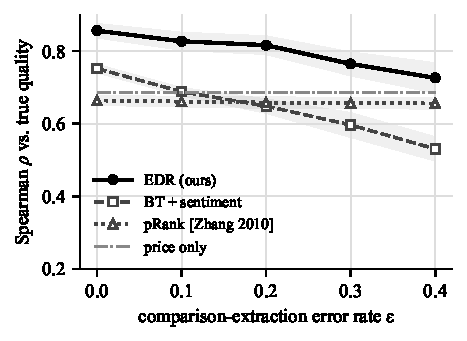
\includegraphics[width=\linewidth]{breakeven.pdf}
\captionof{figure}{Break-even: ranking quality as comparison extraction gets noisier ($\gamma=0.8$).}\label{fig:be}
\end{minipage}
\end{figure}

\paragraph{Findings so far.}
\begin{itemize}
\item \textbf{EDR} (Table~\ref{tab:e1}) ties with pRank and sentiment when reviewers judge absolutely ($\gamma=0$, within one sd) and is the best ranker when
sentiment is price-relative ($\gamma\ge0.5$), where pRank falls from \pRankGzero{} to \pRankGhigh{}. PageRank and HITS mostly measure popularity.
\item \textbf{Break-even} (Figure~\ref{fig:be}): EDR stays clearly above ranking by price up to $\varepsilon=0.3$; at $\varepsilon=0.4$ the margin
(\MarginHigh{}) is within noise. BT + sentiment falls to the price baseline already at $\varepsilon\approx0.1$. This gives an accuracy target
for comparative extraction.
\end{itemize}

\paragraph{First real-data check} (Table~\ref{tab:real}; \NReviews{} reviews, phones with ${\ge}10$ reviews). Of \NLinkedComps{} linked
comparisons in buyer reviews, \NEdgesOld{} target the reviewer's older phone, \NEdgesBrand{} a brand and only \NEdgesCatCat{} another current phone,
so PageRank, HITS and Bradley--Terry give no ranking yet and EDR falls back to its joint estimate of $\gamma$. Price ranking points negative for battery (\RealPriceBattery{}, 95\% CI
\RealPriceBatteryCI) and camera (\RealPriceCamera{}, \RealPriceCameraCI), the direction the simulation predicts, but both intervals include zero;
sentiment tracks screen brightness (\RealSentScreen). The rankers are not yet separable; head-to-head evidence must come from expert articles.
\begin{table}[h]\centering\small\setlength{\tabcolsep}{3.5pt}
\caption{Real data: Spearman $\rho$ (95\% bootstrap CI) against spec-sheet values; $n$ = phones.}\label{tab:real}
% generated by report/make_tables.py from results/ — do not edit
\begin{tabular}{@{}llcccc@{}}
\toprule
Aspect & Proxy ($n$) & Price only & Sentiment & pRank & EDR \\
\midrule
Battery & mAh (23) & $-$0.10 {\scriptsize[$-$0.50, 0.35]} & 0.04 {\scriptsize[$-$0.36, 0.46]} & 0.06 {\scriptsize[$-$0.32, 0.45]} & 0.06 {\scriptsize[$-$0.31, 0.45]} \\
Screen & peak nits (21) & 0.63 {\scriptsize[0.18, 0.91]} & 0.66 {\scriptsize[0.40, 0.83]} & 0.66 {\scriptsize[0.40, 0.84]} & 0.55 {\scriptsize[0.11, 0.81]} \\
Camera & main MP, weak (35) & $-$0.30 {\scriptsize[$-$0.65, 0.09]} & 0.24 {\scriptsize[$-$0.04, 0.48]} & 0.23 {\scriptsize[$-$0.04, 0.47]} & 0.18 {\scriptsize[$-$0.15, 0.47]} \\
\bottomrule
\end{tabular}

\end{table}

%==================================================================================================
\section{Next steps}
\begin{itemize}
\item \textbf{Data.} Obtain VCOM; collect lab benchmarks for a subset; annotate the gold comparative set.
\item \textbf{Extraction.} LLM silver labels vs.\ rules, distilled into a PhoBERT extractor; quintuple F1 on VCOM and gold;
\textbf{measure $\varepsilon$} to place each extractor on the break-even curve.
\item \textbf{Ranking on real data.} Add expert-article comparisons to the graph; evaluate all rankers per aspect against spec proxies
and benchmarks (Spearman, Kendall $\tau$, NDCG@10, bootstrap CIs).
\item \textbf{Deliverables.} Final report, slides, and a demo (aspect $\to$ ranked phones, rank intervals, evidence per comparison).
\end{itemize}

%==================================================================================================
{\fontsize{8}{9.6}\selectfont
\bibliographystyle{iclr2027_conference}
\bibliography{refs}}

\end{document}
